\documentclass[11pt]{article}

\usepackage{report}

\usepackage[utf8]{inputenc} % allow utf-8 input
\usepackage[T1]{fontenc}    % use 8-bit T1 fonts
\usepackage[colorlinks=true, linkcolor=black, citecolor=blue, urlcolor=blue]{hyperref}       % hyperlinks
\usepackage{url}            % simple URL typesetting
\usepackage{booktabs}       % professional-quality tables
\usepackage{amsfonts}       % blackboard math symbols
\usepackage{nicefrac}       % compact symbols for 1/2, etc.
\usepackage{microtype}      % microtypography
\usepackage{lipsum}		% Can be removed after putting your text content
\usepackage{graphicx}
\usepackage{natbib}
\usepackage{doi}
\setcitestyle{aysep={,}}



\title{Toxic Comments Classification}

\author{Aarav Varshney and Argha Chakrabarty\\
\AND
\AND
	Ashoka University\\
}

% Uncomment to remove the date
\date{December 2021}

% Uncomment to override  the `A preprint' in the header
\renewcommand{\headeright}{Project Report}
\renewcommand{\undertitle}{Project Report}
\renewcommand{\shorttitle}{}

%%% Add PDF metadata to help others organize their library
%%% Once the PDF is generated, you can check the metadata with
%%% $ pdfinfo template.pdf
% \hypersetup{
% pdftitle={A template for the arxiv style},
% pdfsubject={q-bio.NC, q-bio.QM},
% pdfauthor={David S.~Hippocampus, Elias D.~Striatum},
% pdfkeywords={First keyword, Second keyword, More},
% }

\begin{document}
\maketitle

\newpage
\tableofcontents
\thispagestyle{empty}

\newpage
\thispagestyle{empty}

\setcounter{page}{1}
\section{Introduction}
The project presents an application of NLP to classify texts posted on online platforms as
comments as either toxic or non-toxic. While social media is a great medium for sharing opinions,
it is more and more being used to bully and harass people. This project aims to classify such comments
and hopefully make social media a bit more welcoming. We study the impact of tf-idf and SVMs, Decision Trees, Naive Bayes and CNNs.
We evaluated our approaches on comments from the \href{https://www.kaggle.com/c/jigsaw-toxic-comment-classification-challenge}{Kaggle Toxic Comments Classification Challenge}. Additionally
we host the classifier so that users can interact with it.


\section{Literature Survey}
\label{sec:headings}
This are several papers already published on the topic of Toxic Comments Classification. This was helpful for us to understand the topic and the way experts have approached it.
We have used the following papers for our analysis: 
\subsection{Toxic Comment Classification by Zaher et al.}
The authors used Naive Bayes (as benchmark), RNN and LSTM to classify toxic comments. They trained the classifier on the same kaggle dataset. 
	\begin{tabular}{cc}
		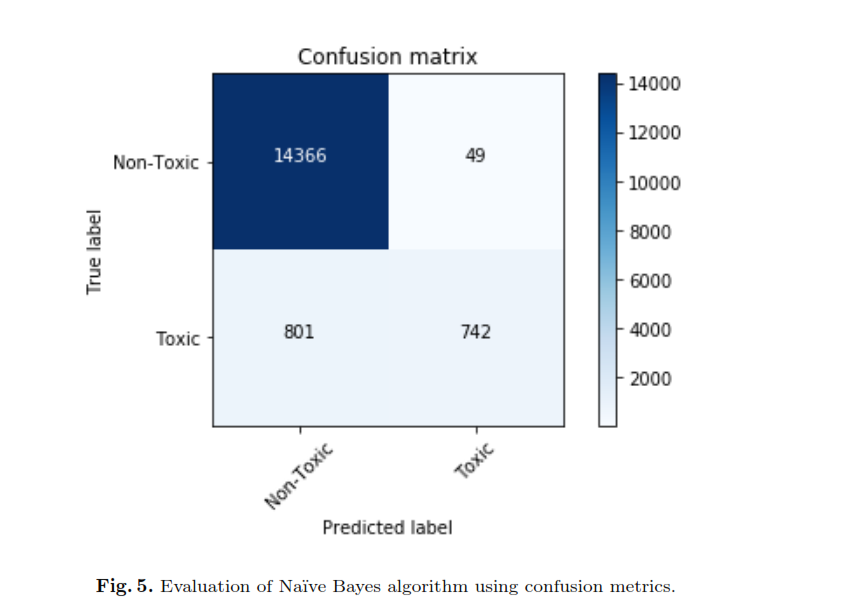
\includegraphics[width=85mm]{figs/zaher_bayes.png} & 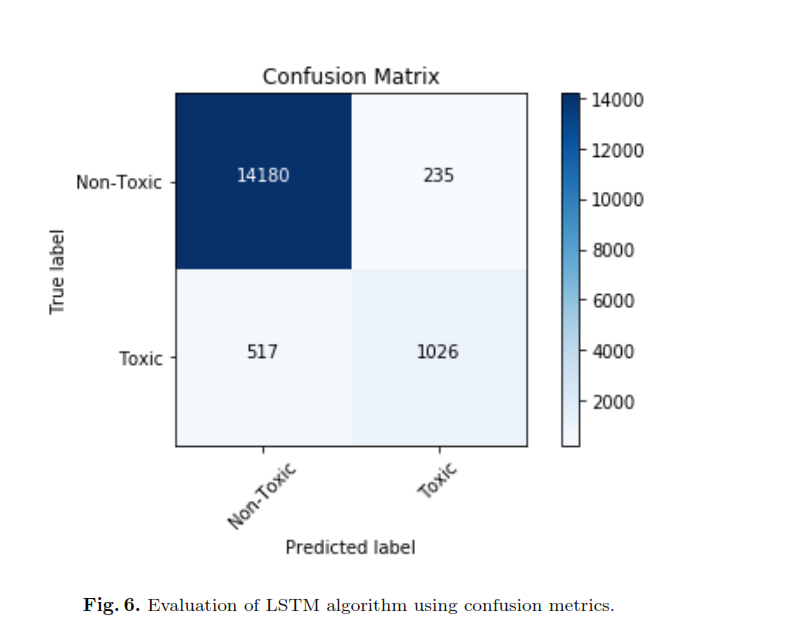
\includegraphics[width=85mm]{figs/zaher_lstm.png} \\
	\end{tabular}
The results showed that LSTM has an almost 20\% increase in True Positive Rate (TRP) which means that among all the identified toxic comments
LSTM has 20\% more sensitivity in correct assignment of the comments. Furthemore there was an increase in Recall and F1 score when using LSTM.

\subsection{A Machine Learning Approach to Comment Toxicity Classification by Navoneel Chakrabarty}
The authors solved the problem of multi-label classification rather than binary and further classified toxic comments as hate, toxic, severelytoxic and so on. Two approaches were used for 3 labels each out of 6 labels. The authors used Bag of words using Word count vectorizer and then the tf-idf transformer which is finally used to train. Support Vector Machine (SVM) classifier with 100 as maximum iterations and C as 1.0. Whereas for the other three labels, decision tree classifier was used instead.
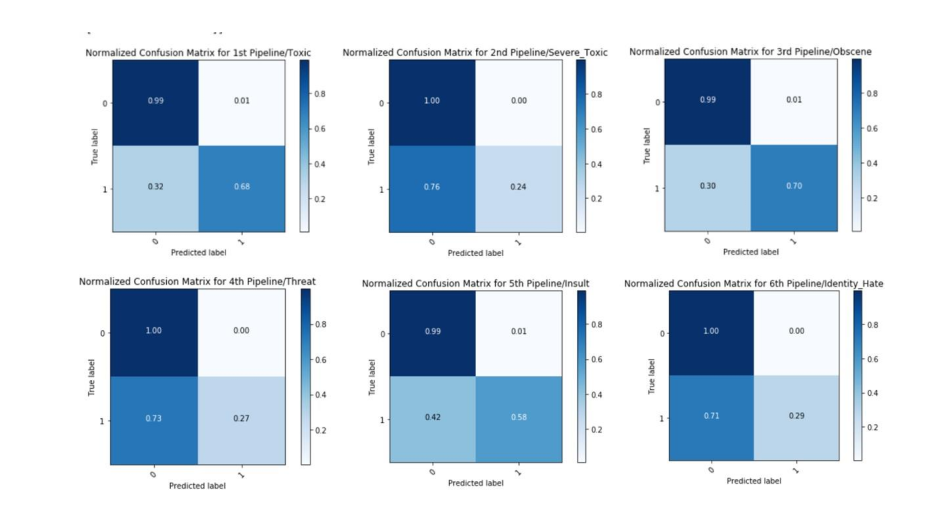
\includegraphics[scale=0.9]{figs/chakra_all.png}
The paper claims that this apporach performs better than LSTM and Naive Bayes and the results validates this claim. We want to validate this claim on binary classification.
\section{Project Description and goals}
\section{Dataset Specification}
Our dataset had 159571 comments, with each comment labelled as toxic, severe toxic, obscene, threat, insult, identity hate or none of 'em. The length of each comment varied from 10 words to 1200 words. To make it easier for us to train the model we chose comments with word count less than 600 as 132327 comments were under 600 words, and the number seemed good enough for the purposes of this project.
\begin{center}
	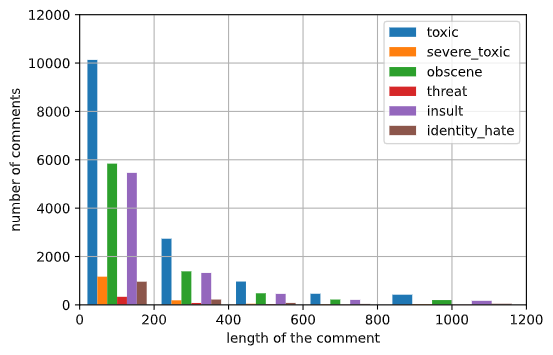
\includegraphics[scale=0.5]{figs/distribution.png}
\end{center}
Due to various constraints we decided to go with a binary classifier rather than a multilabel classifier. For this purpose, we created added a new column, istoxic which labels itself 1 if the comment is toxic and 0 if it isn't.\\
The dataset contained a lot of punctuations and numbers which didn't really contributed to the overall sentiment or toxicity of the comment and hence were removed.\\
Afterwards we first lemmetized, and then stemmed each comment and removed any stop words present. 
\begin{center}
	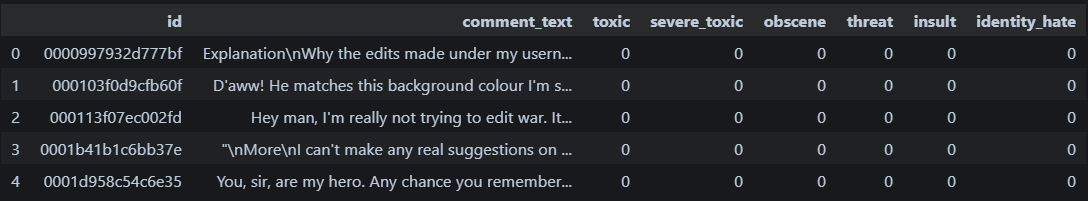
\includegraphics[scale=0.35]{figs/data_set.png}
\end{center}
\section{Methods, experiments and explanation, schematics}
\section{Implementation details}
After the data is read, we select only comments with less than 600 words in it, and label each comment as toxic or not depending on the preexisting labels. nltk's wordnet module is used for stemming and lemmetizeing each comment after removing all the punctuations and numbers along with any other redundant utf-8 characters. After all the comments are cleaned, we use Tfidf word embedding to vectorize our comments so that we can use 'em for training our model. TfidfVectorizer is used as is from the scikit-learn module. The test to train split ratio is 3:1. Then we trained our model on various models, nameley SVM, Logistic Regression, Naive Bayes and decision trees. We trained the model on a laptop with i5-8520U and 16 gigs of RAM. We also trained a multi-label model using Binary Relevence from scikit-multilearn module which is built on top of scikit-learn eco-system and provides multi label classification. After training, we decided to deploy our model for demo purposes. Since we used python for our project, we decided to go with a simple FastAPI server. We created a pipeline with two stages, the first one vectorizing any input text and at the stage the actual fitting or prediction occurs. To save the model we pickle the pipeline object using python's in-built pickle library and write the raw binary data onto a file. Afterwards, the file is un-pickled at the server-side and a single string array is given to it for prediction. The API takes a single string as it's payload and returns the predicted outcome as it's response. The user has to create a POST request with the comment as the payload and we return whether the comment is toxic or not in the response body. Lastly we deployed the whole thing in a heroku server. You can take a look at the API at this link :- \url{https://iml-tox-det.herokuapp.com/docs} (please keep in mind that we are using a free server, it might take some time to start). We also went on and created a frontend website that uses the api: \url{https://adoring-bell-52f360.netlify.app} (the name is generated by netlify)
\section{Observations}
\subsection{Binary Classifier SVM}
Confusion Matrix:
\begin{center}
	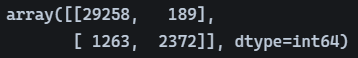
\includegraphics[scale=0.75]{figs/conf_bSVM.png}
\end{center}
Other metrics
\begin{center}
	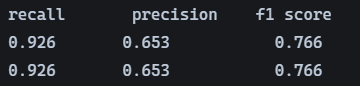
\includegraphics[scale=0.75]{figs/rpf_bSVM.png}	
\end{center}


\subsection{Multilabel Classifier SVM}

\subsection{Logistic Regression}
Confusion Matrix:
\begin{center}
	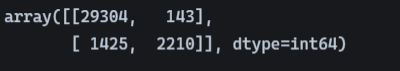
\includegraphics[scale=0.75]{figs/conf_LR.png}
\end{center}
Other metrics
\begin{center}
	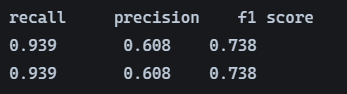
\includegraphics[scale=0.75]{figs/rpf_LR.png}	
\end{center}

\subsection{Naive Bayes}
Confusion Matrix:
\begin{center}
	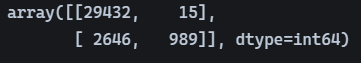
\includegraphics[scale=0.75]{figs/conf_NB.png}
\end{center}
Other metrics
\begin{center}
	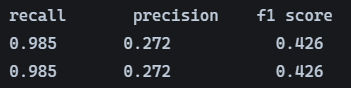
\includegraphics[scale=0.75]{figs/rpf_NBB.png}	
\end{center}

\subsection{Decision Trees}
Confusion Matrix:
\begin{center}
	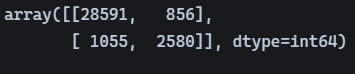
\includegraphics[scale=0.75]{figs/conf_DT.png}
\end{center}
Other metrics
\begin{center}
	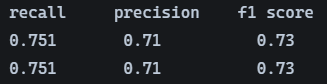
\includegraphics[scale=0.75]{figs/rpf_DT.png}	
\end{center}

\section{Conclusions and future directions}
\section{Examples of citations, figures, tables, references}
\label{sec:others}

\subsection{Citations}
Citations use \verb+natbib+. The documentation may be found at
\begin{center}
	\url{http://mirrors.ctan.org/macros/latex/contrib/natbib/natnotes.pdf}
\end{center}

Here is an example usage of the two main commands (\verb+citet+ and \verb+citep+): Some people thought a thing \citep{kour2014real, hadash2018estimate} but other people thought something else \citep{kour2014fast}. Many people have speculated that if we knew exactly why \citet{kour2014fast} thought this\dots

\subsection{Figures}
\lipsum[10]
% See Figure \ref{fig:fig1}.
Here is how you add footnotes. \footnote{Sample of the first footnote.}
\lipsum[11]

% \begin{figure}
% 	\centering
% 	\fbox{\rule[-.5cm]{4cm}{4cm} \rule[-.5cm]{4cm}{0cm}}
% 	\caption{Sample figure caption.}
% 	\label{fig:fig1}
% \end{figure}

\subsection{Tables}
See awesome Table~\ref{tab:table}.

The documentation for \verb+booktabs+ (`Publication quality tables in LaTeX') is available from:
\begin{center}
	\url{https://www.ctan.org/pkg/booktabs}
\end{center}


\begin{table}
	\caption{Sample table title}
	\centering
	\begin{tabular}{lll}
		\toprule
		\multicolumn{2}{c}{Part}                   \\
		\cmidrule(r){1-2}
		Name     & Description     & Size ($\mu$m) \\
		\midrule
		Dendrite & Input terminal  & $\sim$100     \\
		Axon     & Output terminal & $\sim$10      \\
		Soma     & Cell body       & up to $10^6$  \\
		\bottomrule
	\end{tabular}
	\label{tab:table}
\end{table}

\subsection{Lists}
\begin{itemize}
	\item Lorem ipsum dolor sit amet
	\item consectetur adipiscing elit.
	\item Aliquam dignissim blandit est, in dictum tortor gravida eget. In ac rutrum magna.
\end{itemize}


\bibliographystyle{unsrtnat}
\bibliography{references}  %%% Uncomment this line and comment out the ``thebibliography'' section below to use the external .bib file (using bibtex) .


%%% Uncomment this section and comment out the \bibliography{references} line above to use inline references.
% \begin{thebibliography}{1}

% 	\bibitem{kour2014real}
% 	George Kour and Raid Saabne.
% 	\newblock Real-time segmentation of on-line handwritten arabic script.
% 	\newblock In {\em Frontiers in Handwriting Recognition (ICFHR), 2014 14th
% 			International Conference on}, pages 417--422. IEEE, 2014.

% 	\bibitem{kour2014fast}
% 	George Kour and Raid Saabne.
% 	\newblock Fast classification of handwritten on-line arabic characters.
% 	\newblock In {\em Soft Computing and Pattern Recognition (SoCPaR), 2014 6th
% 			International Conference of}, pages 312--318. IEEE, 2014.

% 	\bibitem{hadash2018estimate}
% 	Guy Hadash, Einat Kermany, Boaz Carmeli, Ofer Lavi, George Kour, and Alon
% 	Jacovi.
% 	\newblock Estimate and replace: A novel approach to integrating deep neural
% 	networks with existing applications.
% 	\newblock {\em arXiv preprint arXiv:1804.09028}, 2018.

% \end{thebibliography}


\end{document}
